\section{Second Member}
\subsection{First Paragraph}
At the beginning, the module seemed to be very bording for me. I thought "Why would anyone care about this complicated kind of planning". However, as the module progressed it all started to make more sense, and the sense of boring started to dissapear. I would definetly say that the weakness of this module is that it started with a sort-of "boring" material, and became more relevant as it progressed. So if I was Max, I would choose a different material that's more connected to Computer programming to start with. As the first semster was mainly based on programming.

\subsection{Comments about the module}
The best parts of this module is the JUnit testing, because it taught me a new way of testing the software without messing up the original code.

What I like about Max is that he's not boring, in other words, he never drives you to feel sleepy in class. I guess this is due to his random sense of humor, and maybe to confiedence hes has while presenting. Moreover, as he's a democratic teacher, which is key aspect of his personality, which makes students feel more important. Furthermore, he's young, so I feel he's more connected to the students and understand our mentality.

\subsection{Selfie with Max}
\begin{figure}[h]
\caption{Selfie with Max}
\centering
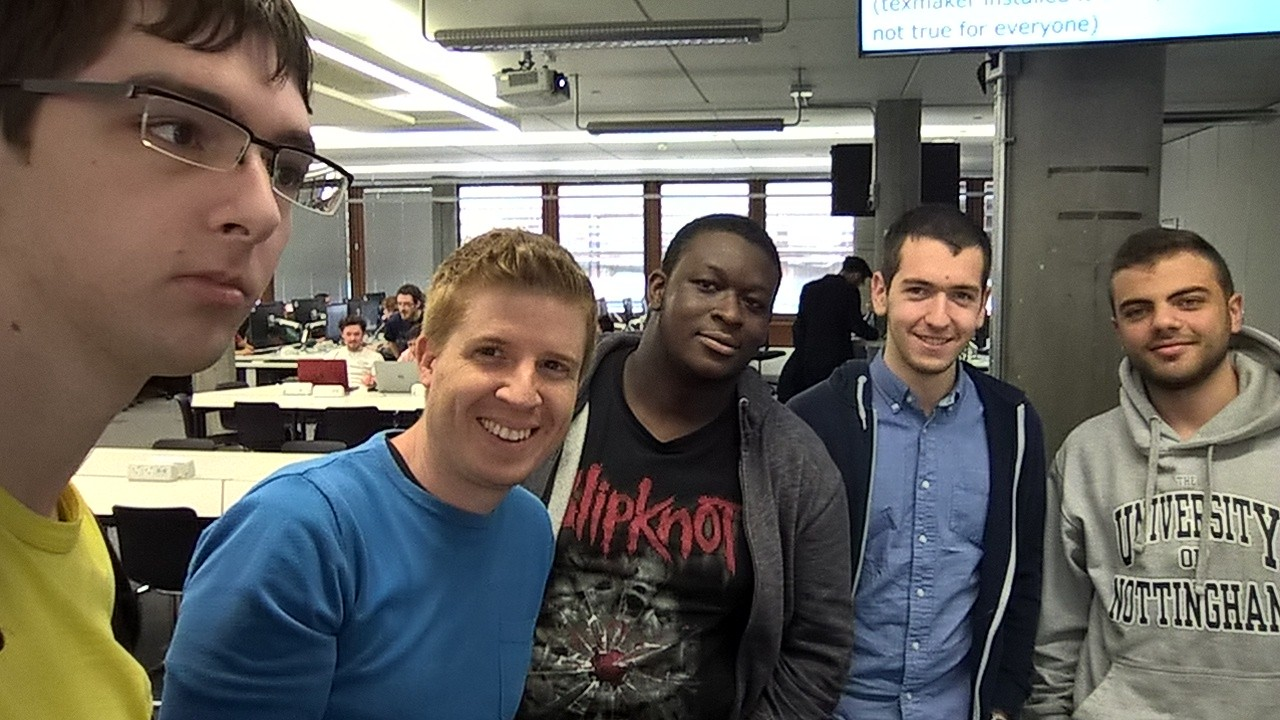
\includegraphics[width=0.5\textwidth]{pic.jpg}
\label{fig:selfie}
\end{figure}

\subsection{What I have learned in this module}
I have learned many useful things in this module, such as:
\begin{itemize}
\item How to plan for a software before building it, in order to build better software that's maintainable and user-friendly
\item Planning Tests throughout the building cycle, to ensure that all standards, requirements and specifications are being met.
\item Using JUnit to do automatic code testing, which saves alot of time instead of doing it manually.
\end{itemize}
